\documentclass[conference]{IEEEtran}

\usepackage{cite}
\usepackage{amsmath,amssymb,amsfonts}
\usepackage{algorithmic}
\usepackage{algorithm}
\usepackage{graphicx}
\usepackage{textcomp}
\usepackage{xcolor}
\usepackage{url}
\usepackage{array}
\usepackage{tikz}
\usepackage{pgfplots}
\pgfplotsset{compat=1.18}
\usetikzlibrary{arrows.meta,bending,positioning}

% Override IEEEtran's default \normalsize (10pt) affiliation font to \small (9pt).
% At 10pt, "Dept. of Computer Science and Engineering" is ~65mm wide per block;
% three blocks (195mm) exceed the 177.8mm text width and force a 2+1 wrap.
% At 9pt, each block is ~58mm; three blocks (174mm) fit in one row.
\makeatletter
\def\@IEEEauthorblockAstyle{\normalfont\small}
\makeatother

\begin{document}

\title{eBPF-Driven Dual-Track Control Plane for FSM-Gated Autonomous Remediation of Containerized Workloads}

\author{%
\IEEEauthorblockN{Pranav Negi}
\IEEEauthorblockA{\textit{Dept. of Computer Science and Engineering}\\
\textit{PES University}\\
Bengaluru, India\\
pes2ug23cs429@pesu.pes.edu}
\and
\IEEEauthorblockN{Reema Sarkar}
\IEEEauthorblockA{\textit{Dept. of Computer Science and Engineering}\\
\textit{PES University}\\
Bengaluru, India\\
pes2ug23cs471@pesu.pes.edu}
\and
\IEEEauthorblockN{Animesh Giri}
\IEEEauthorblockA{\textit{Dept. of Computer Science and Engineering}\\
\textit{PES University}\\
Bengaluru, India\\
animeshgiri@pes.edu}
}

\maketitle

\begin{abstract}
Containerized workloads mix stateful databases and stateless services whose failure semantics differ fundamentally, yet most remediation frameworks still apply a single recovery policy to both. This uniformity ignores the distinct safety requirements each workload type carries. We present a dual-track control plane that separates stateless and stateful workloads into independent eBPF-driven remediation pipelines. Stateless workloads are managed through a confidence-based decision DAG; stateful workloads incorporate a finite-state machine (FSM), shadow execution, and a WebAssembly (WASM) policy layer that enforces safe action sequencing before irreversible recovery operations. We evaluated the framework on 9,132 execution traces and 90 controlled fault-injection experiments across PostgreSQL, Redis, MySQL, and Nginx container workloads. A stateful divergence rate of 1.93\% confirms that accumulated FSM state materially changes dispatch outcomes relative to a memoryless baseline. Mean time to checkpoint dispatch ranged from 10.40 to 11.54\,s; WASM policy evaluation added 27\,$\mu$s and shadow execution 8\,$\mu$s per cycle; both are negligible within the 5\,s budget. Workload-aware control plane separation is both feasible and measurably necessary for safe autonomous remediation where stateful and stateless workloads coexist.
\end{abstract}

\begin{IEEEkeywords}
autonomic computing, eBPF, container remediation, finite state machines, shadow execution, safe remediation
\end{IEEEkeywords}

\section{Introduction}
\label{sec:intro}

Not every container fails the same way. If an \texttt{nginx} worker crashes, you simply restart it---no harm done. But a \texttt{postgres} instance under heavy I/O is a different story entirely: it needs a flush first, then a checkpoint, in that exact order. Jump ahead or skip a step, and you risk corrupting transactions that haven't committed yet. Large-scale autonomous resource management is well-established at this point~\cite{b14}, but the frameworks available today tend to apply a single blanket policy across all containers~\cite{b1}, or they leave the decision to human operators, who cannot match the speed of continuous eBPF-level observability~\cite{b6}.

Thanks to eBPF, per-process kernel telemetry is now cheap and continuous, requiring zero changes to the application itself~\cite{b6}. But just collecting signals is not enough to guarantee safe remediation. When you are dealing with stateful workloads, three things need to be in place: there has to be an audit step before any checkpoint fires; something has to block irreversible actions until the right sequence is followed; and each cycle needs to check whether the FSM's accumulated state actually influences what gets dispatched, compared with a baseline that has no memory.

Right now, nothing out there checks all three boxes at once. Kubernetes's built-in remediation mechanisms~\cite{b1} do not enforce any ordering between flush and checkpoint. eBPF observability layers~\cite{b6} give you excellent signal granularity, but they do not tell you what to do with those signals safely. And as Bronson et al.~\cite{b15} showed, systems can slip into degraded states that a memoryless recovery policy is unable to reverse. The gap is architectural.

The dual-track control plane we describe here tackles all three. Our contributions are as follows: (1)~a dual-track eBPF architecture with independent Type~S and Type~F pipelines (\S\ref{sec:arch}, \S\ref{sec:types}, \S\ref{sec:typef}); (2)~a five-state FSM paired with a WASM policy layer that enforces action sequencing before any irreversible checkpoint can fire; (3)~real/shadow execution that turns divergence into a first-class, continuously observable metric; and (4)~a six-metric evaluation (M1--M6) across 9,132 traces and 90 fault-injection episodes, along with an ablation that shows FSM gating is strictly necessary (\S\ref{sec:eval}).

\section{Background and Related Work}
\label{sec:background}

\textbf{Autonomic computing and MAPE-K.} Kephart and Chess~\cite{b8} defined the MAPE-K loop~\cite{b7} as the standard self-managing architecture. Our design maps onto it directly: eBPF probes serve as Monitor, per-track scorers as Analyse, the FSM-gated DAG as Plan, and the action executor as Execute---split into two independent branches on a shared event bus.

\textbf{Kubernetes operators.} Kubernetes's built-in controllers and Pod Autoscalers~\cite{b1} remediate via pod restarts and replica scaling only; state-machine monitoring~\cite{b10} adds anomaly detection but not safe recovery sequencing. Neither operates at the I/O-path signal level---precisely where stateful workload risk materialises.

\textbf{eBPF and observability.} BCC~\cite{b6} makes kernel-level probes cheap enough to run continuously. Our implementation attaches kprobes on \texttt{blk\_account\_io\_start/done}, kretprobes on \texttt{vfs\_write/read}, and tracepoints on \texttt{sys\_enter\_umount/mount}---I/O and filesystem visibility requiring no application modification. Basiri et al.~\cite{b3} formalise fault injection as a technique to expose systemic weaknesses; the M3 harness applies the same idea at the signal level, driving the full FSM recovery path synthetically.

\textbf{Formal methods and shadow execution.} TLA+~\cite{b9} supports formal verification of state-machine properties at design time; the FSM here enforces the same constraints at runtime via executable guards. Each reconcile cycle also runs on a fresh throwaway FSM copy alongside the live path; any difference in the dispatched action is logged as M2. WebAssembly isolates each module's memory and execution by design~\cite{b11}, so a WASM module~\cite{b4} acts as the second enforcement gate at the execution boundary, independent of the FSM.

\section{System Architecture}
\label{sec:arch}

\subsection{Overview}

Fig.~\ref{fig:arch} shows the full pipeline. Both tracks follow the same path (kernel probes $\rightarrow$ perf buffer $\rightarrow$ comm-filtered listener $\rightarrow$ StateStore $\rightarrow$ scorer $\rightarrow$ DAG $\rightarrow$ executor); Type~F inserts an FSM and WASM policy layer before the executor. Every reconcile cycle runs twice: real path (live FSM, dispatches) and shadow path (fresh FSM, suppressed); disagreements are logged to a divergence log. eBPF probes are kernel-global; attribution matches each event's \texttt{comm} field against a static allow-list---unmatched events are dropped before the StateStore.

\begin{figure}[!t]
\centering
\begin{tikzpicture}[
  font=\scriptsize,
  box/.style={draw, rounded corners=2pt, minimum width=2.70cm,
              minimum height=0.48cm, align=center, fill=white},
  sbox/.style={draw, rounded corners=2pt, minimum width=2.70cm,
               minimum height=0.48cm, align=center, fill=gray!10},
  arr/.style={->, >=Stealth[length=4pt,width=2pt], line width=0.7pt},
  wide/.style={draw, rounded corners=2pt, minimum width=5.85cm,
               minimum height=0.48cm, align=center, fill=white},
]
% ---- Kernel layer (two-line node so text fits in column width) ----
\node[wide, minimum height=0.72cm] (ebpf) at (0, 5.40)
  {\textbf{Kernel eBPF Probes}\\
   \texttt{process\_exit} $\cdot$ \texttt{tcp\_connect} $\cdot$ \texttt{blk\_io} $\cdot$ \texttt{vfs}};

% ---- perf buffer ----
\node[wide] (buf) at (0, 4.42) {perf ring buffer (per track)};
\draw[arr] (ebpf) -- (buf);

% ---- Track column headers (outside arrow paths) ----
\node[font=\tiny\bfseries\itshape] at (-2.10, 3.94) {Type~S~~Stateless};
\node[font=\tiny\bfseries\itshape] at ( 2.10, 3.94) {Type~F~~Stateful};

% ---- Two tracks side by side ----
\node[sbox] (esS)  at (-1.55, 3.58) {EventListener~+~filter};
\node[sbox] (esF)  at ( 1.55, 3.58) {EventListener~+~filter};
\node[sbox] (ssS)  at (-1.55, 2.74) {StateStore (60\,s)};
\node[sbox] (ssF)  at ( 1.55, 2.74) {StatefulStateStore (60\,s)};
\node[sbox] (scS)  at (-1.55, 1.90) {Confidence Scorer~S};
\node[sbox] (scF)  at ( 1.55, 1.90) {Confidence Scorer~F};
\node[sbox] (dagS) at (-1.55, 1.06) {Threshold DAG};
\node[sbox] (dagF) at ( 1.55, 1.06) {FSM-Gated DAG};
\node[box]  (pol)  at ( 1.55, 0.22) {WASM Policy Layer};

% Vertical arrows within each track
\foreach \a/\b in {buf/esS, esS/ssS, ssS/scS, scS/dagS}
  \draw[arr] (\a) -- (\b);
\foreach \a/\b in {buf/esF, esF/ssF, ssF/scF, scF/dagF, dagF/pol}
  \draw[arr] (\a) -- (\b);

% ---- Shared action executor ----
\node[wide, minimum height=0.64cm] (exec) at (0,-0.80)
  {Action Executor\\
   \textit{real path: executed\quad shadow path: suppressed}};
\draw[arr] (dagS) -- (exec);
\draw[arr] (pol)  -- (exec);

% ---- Output ----
\node[wide] (trace) at (0,-1.72)
  {TraceLogger $\rightarrow$ execution traces \,$\cdot$\, divergence log};
\draw[arr] (exec) -- (trace);

% Vertical divider between the two tracks
\draw[dashed, gray!60] (0, 3.70) -- (0, -0.20);
\end{tikzpicture}
\vspace{2pt}
\caption{Dual-track control plane. Type~S and Type~F share the eBPF event bus but run independent scorers. Type~F adds an FSM-gated DAG and WASM policy layer. Both a real path (live FSM, executed) and a shadow path (fresh FSM, suppressed) run each cycle; divergences increment M2.}
\label{fig:arch}
\end{figure}

\section{Type S: Stateless Control Plane}
\label{sec:types}

\subsection{Kernel Probes and Confidence Scoring}

Type~S attaches a tracepoint on \texttt{sched\_process\_exit} and a kprobe on \texttt{tcp\_connect} capturing all connection attempts; elevated connection activity in the window is treated as a proxy for connectivity stress. Per-signal scores for container $c$ and window $W$:

\begin{equation}
s_{\mathrm{pe}}(c, W) = \sigma_{\mathrm{pe}} \cdot \mathbb{1}\!\left[n_{\mathrm{pe}}(c, W) > 0\right]
\label{eq:spe}
\end{equation}

\begin{equation}
s_{\mathrm{tc}}(c, W) = \min\!\left(\frac{n_{\mathrm{tc}}(c, W)}{\theta_{\mathrm{tc}}},\, 1\right) \cdot \sigma_{\mathrm{tc}}
\label{eq:stc}
\end{equation}

Parameters: $\sigma_{\mathrm{pe}} = 0.95$, $\sigma_{\mathrm{tc}} = 0.90$, $\theta_{\mathrm{tc}} = 5$. Scaling TCP activity by count means a single connection attempt will not cross the action threshold. The combined score:

\begin{equation}
\rho_S(c, W) = \max(s_{\mathrm{pe}}(c, W),\, s_{\mathrm{tc}}(c, W))
\label{eq:rhoS}
\end{equation}

\subsection{Decision DAG}

Type~S maps $\rho_S$ to three actions. Thresholds: $\tau_{\mathrm{restart}} = 0.80$, $\tau_{\mathrm{reschedule}} = 0.95$:

\begin{equation*}
\delta_S(c) =
\begin{cases}
\texttt{reschedule} & \text{if } \rho_S \geq \tau_{\mathrm{reschedule}} \\
\texttt{restart}    & \text{if } \tau_{\mathrm{restart}} \leq \rho_S < \tau_{\mathrm{reschedule}} \\
\texttt{no\_action} & \text{if } \rho_S < \tau_{\mathrm{restart}}
\end{cases}
\end{equation*}

Both actions are reversible by design. No FSM is required here---stateless workloads do not carry on-disk state that an ill-timed restart could damage. Because every restart returns the container to an identical initial state, there is no observable lifecycle---no audit phase, no sequencing constraint---that would require persistent memory across cycles.


\section{Type F: Stateful Control Plane}
\label{sec:typef}

\subsection{Kernel Probes and Confidence Scoring}

Type~F attaches kprobes on \texttt{blk\_account\_io\_start/done}, kretprobes on \texttt{vfs\_write/read}, and tracepoints on \texttt{sys\_enter\_umount/mount}. These produce \texttt{blk\_io\_latency}, VFS error, and volume mount events. Let $n_h(c, W)$ be the count of high-latency I/O events (\texttt{latency\_us} $\geq \Lambda = 10{,}000\,\mu$s), $n_{\mathrm{vfs}}(c, W)$ the VFS error count, and $\mathrm{vol}(c, W) = 1$ when an unresolved mount loss is present in the window.

\begin{equation}
s_{\mathrm{io}}(c, W) = \min\!\left(\frac{n_h(c, W)}{\theta_{\mathrm{io}}},\, 1\right) \cdot \sigma_{\mathrm{io}}
\label{eq:sio}
\end{equation}

\begin{equation}
s_{\mathrm{vfs}}(c, W) = \min\!\left(\frac{n_{\mathrm{vfs}}(c, W)}{\theta_{\mathrm{vfs}}},\, 1\right) \cdot \sigma_{\mathrm{vfs}}
\label{eq:svfs}
\end{equation}

\begin{equation}
s_{\mathrm{vol}}(c, W) = \sigma_{\mathrm{vol}} \cdot \mathbb{1}\!\left[\mathrm{vol}(c, W)\right]
\label{eq:svol}
\end{equation}

Parameters: $\theta_{\mathrm{io}} = 5$, $\sigma_{\mathrm{io}} = 0.85$, $\theta_{\mathrm{vfs}} = 3$, $\sigma_{\mathrm{vfs}} = 0.88$, $\sigma_{\mathrm{vol}} = 0.97$. The combined score is:

\begin{equation}
\rho_F(c, W) = \max(s_{\mathrm{io}}(c, W),\, s_{\mathrm{vfs}}(c, W),\, s_{\mathrm{vol}}(c, W))
\label{eq:rhoF}
\end{equation}

\subsection{Five-State FSM}

Table~\ref{tab:fsm} and Fig.~\ref{fig:fsm} give the full transition relation. The FSM persists across cycles, resetting only after full recovery. The five states correspond to the five distinct checkpoints a safe stateful recovery must pass through: normal operation (Healthy), first signal detection (Degraded), flush-and-audit completion (Audited), checkpoint dispatch (Repairing), and confirmed recovery (Recovered)---collapsing any two adjacent states would either remove the audit gate or make premature C\&R dispatch undetectable. Its central constraint: \texttt{checkpoint\_and\_restart} (CRIU~\cite{b2}) cannot fire in the same cycle that first issues \texttt{flush\_io\_queue}. In Algorithm~\ref{alg:reconcile}, step~4b fires the \texttt{audit} transition within the same call that step~4a downgrades C\&R to flush---making C\&R reachable only on the following cycle, enforcing a minimum 5\,s gap between detection and checkpoint dispatch.


\begin{table}[!t]
\caption{TYPE F FSM TRANSITION RELATION.}
\label{tab:fsm}
\centering
\renewcommand{\arraystretch}{1.20}
\resizebox{0.97\columnwidth}{!}{%
\begin{tabular}{llll}
\hline
\textbf{From} & \textbf{Trigger} & \textbf{To} & \textbf{Condition} \\
\hline
Healthy   & \texttt{degrade}         & Degraded  & $\rho_F \geq \tau_{\mathrm{flush}}$ \\
Degraded  & \texttt{audit}           & Audited   & \texttt{flush\_io\_queue} executed \\
Degraded  & \texttt{degrade}         & Degraded  & score re-confirmed; state held \\
Audited   & \texttt{approve\_repair} & Repairing & \texttt{checkpoint\_and\_restart} approved \\
Audited   & \texttt{degrade}         & Degraded  & fault worsens during audit phase \\
Repairing & \texttt{recover}         & Recovered & action succeeded \\
Repairing & \texttt{degrade}         & Degraded  & repair fails; restart fault path \\
Recovered & \texttt{heal}            & Healthy   & $\rho_F < \tau_{\mathrm{flush}}$ \\
Recovered & \texttt{degrade}         & Degraded  & $\rho_F \geq \tau_{\mathrm{flush}}$ (re-fault) \\
\hline
\end{tabular}%
}
\end{table}

\begin{figure}[!t]
\centering
\begin{tikzpicture}[
  ->, >=Stealth[length=4pt,width=2pt], line width=0.7pt,
  st/.style={draw, rounded corners=3pt,
             minimum width=1.65cm, minimum height=0.50cm,
             align=center, font=\scriptsize\bfseries, fill=white},
  lbl/.style={font=\tiny, fill=white, inner sep=1pt, sloped},
  scale=0.96, transform shape,
]
% Pentagon layout: radius=2.15, clockwise from 90 deg
% Angles: Healthy=90, Degraded=18, Audited=306, Repairing=234, Recovered=162
\node[st] (H) at ( 0.000,  2.150) {Healthy};
\node[st] (D) at ( 2.044,  0.665) {Degraded};
\node[st] (A) at ( 1.265, -1.739) {Audited};
\node[st] (R) at (-1.265, -1.739) {Repairing};
\node[st] (V) at (-2.044,  0.665) {Recovered};

% --- Forward arcs (clockwise, solid) ---
\draw (H) to[bend left=12]  node[lbl, above right]{degrade}    (D);
\draw (D) to[bend left=12]  node[lbl, right]      {audit}      (A);
\draw (A) to[bend left=12]  node[lbl, below]      {approve\_repair}    (R);
\draw (R) to[bend left=12]  node[lbl, below left] {recover}    (V);
\draw (V) to[bend left=12]  node[lbl, above left] {heal}       (H);

% --- Back-edges (dashed, gray) ---
% Self-loop on Degraded (exit NE, return SE)
\draw[dashed,gray!70] (D.north east)
    to[out=50, in=320, looseness=3.5]
    node[lbl, right=2pt, sloped=false]{\tiny degrade}
    (D.south east);
% Audited -> Degraded (degrade)
\draw[dashed,gray!70] (A) to[bend right=38]
    node[lbl, above right, xshift=4pt, yshift=3pt]{\tiny degrade} (D);
% Repairing -> Degraded (degrade)
\draw[dashed,gray!70] (R) to[out=70, in=230, looseness=0.85]
    node[lbl, above, sloped=false]{\tiny degrade} (D);
% Recovered -> Degraded (re-fault)
\draw[dashed,gray!70] (V) to[bend right=22]
    node[lbl, above]{\tiny degrade} (D);
\end{tikzpicture}
\caption{Type~F five-state FSM. Solid arcs: nominal recovery path. Dashed arcs: recurrence/failure routes back to Degraded. C\&R is only reachable from Audited, enforcing at least one 5\,s gap between detection and checkpoint dispatch.}
\label{fig:fsm}
\end{figure}

\subsection{FSM-Gated Reconciliation and Policy Layer}

\begin{algorithm}
\caption{Type~F FSM-Gated Reconciliation (single container $c$)}
\label{alg:reconcile}
\small
\begin{algorithmic}[1]
\REQUIRE StateStore $\mathcal{S}$, FSM $\mathcal{F}$, container $c$
\ENSURE Decision record with \textit{action} and \textit{blocked\_reason}
\STATE $\rho \leftarrow \rho_F(c, \mathcal{S})$;\ $\mathit{sig} \leftarrow \mathrm{KernelSignals}(\mathcal{S}, c)$;\ $q \leftarrow \mathcal{F}.\mathrm{state}(c)$
\STATE \textit{--- (1) Raw DAG ---}
\IF{$\rho \geq \tau_{\mathrm{escalate}}$}
    \STATE $\mathit{raw} \leftarrow \texttt{escalate}$
\ELSIF{$\rho \geq \tau_{\mathrm{repair}}$}
    \STATE $\mathit{raw} \leftarrow \texttt{C\&R}$
\ELSIF{$\rho \geq \tau_{\mathrm{flush}}$}
    \STATE $\mathit{raw} \leftarrow \texttt{flush}$
\ELSE
    \STATE $\mathit{raw} \leftarrow \texttt{no\_action}$
\ENDIF
\STATE $\mathit{act} \leftarrow \mathit{raw}$
\STATE \textit{--- (2) Reversibility gate ---} \COMMENT{$\mathit{IrreversibleActions} = \{\texttt{volume\_delete}\}$}
\IF{$\mathit{raw} \in \mathit{IrreversibleActions}$}
    \STATE $\mathit{act} \leftarrow \texttt{no\_action}$; set \textit{blocked\_reason}
\ENDIF
\STATE \textit{--- (3) FSM degrade ---}
\IF{$\rho \geq \tau_{\mathrm{flush}}$ \AND $\mathit{act} \neq \texttt{no\_action}$ \AND $q \in \{\textit{Healthy}, \textit{Recovered}\}$}
    \STATE $\mathcal{F}.\mathrm{apply}(c, \texttt{degrade})$;\ $q \leftarrow \mathcal{F}.\mathrm{state}(c)$
\ENDIF
\STATE \textit{--- (4) FSM gates ---}
\IF{$\mathit{act} = \texttt{C\&R}$ \AND $q \neq \textit{Audited}$}
    \STATE $\mathit{act} \leftarrow \texttt{flush}$; set \textit{blocked\_reason} \COMMENT{step~4a: C\&R deferred until Audited}
\ENDIF
\IF{$\mathit{act} = \texttt{flush}$ \AND $q = \textit{Degraded}$}
    \STATE $\mathcal{F}.\mathrm{apply}(c, \texttt{audit})$;\ $q \leftarrow \mathcal{F}.\mathrm{state}(c)$ \COMMENT{step~4b: Degraded $\rightarrow$ Audited}
\ENDIF
\IF{$\mathit{act} = \texttt{C\&R}$ \AND $q = \textit{Audited}$}
    \STATE $\mathcal{F}.\mathrm{apply}(c, \texttt{approve\_repair})$ \COMMENT{Audited $\rightarrow$ Repairing}
\ENDIF
\IF{$\mathit{act} = \texttt{escalate}$ \AND $q \notin \{\textit{Degraded}, \textit{Audited}, \textit{Repairing}\}$}
    \STATE $\mathit{act} \leftarrow \texttt{flush}$; set \textit{blocked\_reason} \COMMENT{escalate gate}
\ENDIF
\STATE \textit{--- (5) Heal ---}
\IF{$\rho < \tau_{\mathrm{flush}}$ \AND $q = \textit{Recovered}$}
    \STATE $\mathcal{F}.\mathrm{apply}(c, \texttt{heal})$ \COMMENT{Recovered $\rightarrow$ Healthy}
\ENDIF
\RETURN $(c,\, \rho,\, \mathit{act},\, \mathit{sig},\, \mathcal{F}.\mathrm{state}(c),\, \mathit{blocked\_reason})$
\end{algorithmic}
\end{algorithm}

Thresholds: $\tau_{\mathrm{flush}} = 0.50$, $\tau_{\mathrm{repair}} = 0.80$, $\tau_{\mathrm{escalate}} = 0.95$. \texttt{C\&R} abbreviates \texttt{checkpoint\_and\_restart}; \texttt{flush} abbreviates \texttt{flush\_io\_queue}; $q = \mathcal{F}.\mathrm{state}(c)$.

On the real path the FSM is mutated in-place; on the shadow path a fresh copy runs and is discarded. A pluggable WASM policy layer~\cite{b4} re-checks FSM sequence constraints as a second enforcement gate; validation is described in \S\ref{sec:limitations}. M6 counts Python-gate suppressions only, as the corpus predates wasmtime activation (Table~\ref{tab:metrics}, footnote~$^{b}$).

\section{Research Metrics and Evaluation Framework}
\label{sec:metrics}

Six metrics are defined over $\mathcal{T}$ (the full trace set), $\mathcal{T}_{\mathrm{real}}$ (real-path subset), and $\mathcal{T}_{\mathrm{active}} = \{t \in \mathcal{T}_{\mathrm{real}} : \mathrm{action}(t) \neq \texttt{no\_action}\}$.

\textbf{Schema validation} (M1, M5):
\begin{align}
M_1 &= \frac{|\{t \in \mathcal{T} : \mathrm{misclassified}(t)\}|}{|\mathcal{T}|} \notag \\
M_5 &= \frac{|\{t \in \mathcal{T} : \mathrm{complete}(t)\}|}{|\mathcal{T}|}
\label{eq:M1M5}
\end{align}
M1 counts records with cross-track signal contamination; M5 counts records with all required explanation fields present (\texttt{why}, \texttt{action}, \texttt{score}, \texttt{kernel\_signals}, \texttt{dag\_pattern}).

\textbf{M2: Divergence Rate.} Fraction of real-path cycles where real and shadow actions disagree:
\begin{equation}
M_2 = \frac{|\{t \in \mathcal{T}_{\mathrm{real}} : a_{\mathrm{real}}(t) \neq a_{\mathrm{shadow}}(t)\}|}{|\mathcal{T}_{\mathrm{real}}|}
\label{eq:M2}
\end{equation}

\textbf{M3: Mean Time to First Checkpoint Dispatch (MTTR proxy).} Mean wall-clock time from fault injection to first C\&R dispatch; this measures decision latency, not service restoration---actual container restart adds 300--1{,}300\,ms depending on workload:
\begin{equation}
M_3 = \frac{1}{|\mathcal{E}|} \sum_{e \in \mathcal{E}} \!\left(t_{\mathrm{cr}}(e) - t_{\mathrm{fault}}(e)\right)
\label{eq:M3}
\end{equation}

\textbf{M4: Reversibility Ratio.} \quad \textbf{M6: Suppression Rate.}
\begin{align}
M_4 &= \frac{|\{t \in \mathcal{T}_{\mathrm{active}} : \mathrm{reversible}(t)\}|}{|\mathcal{T}_{\mathrm{active}}|} \notag \\
M_6 &= \frac{|\{t \in \mathcal{T}_{\mathrm{real}} : \mathrm{suppressed}(t)\}|}{|\mathcal{T}_{\mathrm{real}}|}
\label{eq:M4M6}
\end{align}


\section{Evaluation}
\label{sec:eval}

M1, M2, M4--M6 are derived from the committed trace corpus; M3 uses a synthetic fault-injection harness (\S\ref{sec:m3}).

\subsection{Experimental Setup}

All experiments ran on a single ARM64 workstation (Apple M4, Ubuntu~22.04, Linux~5.15, 8\,GB RAM). Four Docker containers were monitored: \texttt{nginx}~1.29.6 (Type~S), and \texttt{postgres}~18.3, \texttt{redis}~8.6.2, and \texttt{mysql}~9.6.0 (Type~F). Reconcile interval: 5\,s; sliding window: 60\,s (MTTR episodes: 120\,s). All decisions were logged for offline analysis.

\subsection{Trace-Based Metric Results}

$M_1 = 0.0000$, $M_5 = 1.0000$: no trace carried cross-track signals, and all required explanation fields were populated across the full 9,132-record corpus (\texttt{kernel\_signals} is intentionally empty for \texttt{no\_action} decisions and is treated as valid).

Both tracks achieve $M_4 = 1.0000$: all 2,113 Type-S decisions (\texttt{reschedule}) and all 95 Type-F decisions carry \texttt{reversibility="reversible"}. Neither \texttt{volume\_delete} nor \texttt{escalate} was dispatched; \texttt{escalate}'s conditional tag would lower M4 if triggered.

$M_2^\mathrm{F} = M_6^\mathrm{F} = 0.0193$ (44 of 2,282 real stateful cycles); all 44 divergence records appear in the stateful divergence log with the pair \texttt{checkpoint\_and\_restart}$\rightarrow$\texttt{flush\_io\_queue}. On the stateless track, shadow and real paths run the same memoryless DAG: $M_2^\mathrm{S} = 0.0000$, giving $M_2^\mathrm{overall} = 0.0096$. The equality $M_2^\mathrm{F} = M_6^\mathrm{F}$ is not a coincidence---it is structural. Each of the 44 C\&R-eligible episodes produces exactly one M6 cycle (real FSM in Degraded blocks C\&R; shadow issues \texttt{flush}; no divergence) and one M2 cycle (real FSM in Audited approves C\&R; shadow defers to \texttt{flush}; divergence logged).

\subsection{Fault-Injection MTTR Campaign}
\label{sec:m3}

$M_3$ was measured using a dedicated fault-injection harness: eight \texttt{blk\_io\_latency} events (50--54\,ms) are injected into a fresh \texttt{StatefulStateStore} (window 120\,s), reconciling every 5\,s and recording wall time from injection to first C\&R dispatch. This captures the structural two-cycle delay---\texttt{flush} fires in cycle~1 (Healthy$\rightarrow$Degraded$\rightarrow$Audited) and C\&R is approved in cycle~2. Unlike state-perturbation approaches~\cite{b12}, injection here measures decision latency, not latent bugs.

Across three workloads ($N = 30$ episodes each, 90 total; Fig.~\ref{fig:mttr}): \texttt{postgres} $\mu = 10.87$\,s ($\sigma = 0.09$\,s); \texttt{redis} $\mu = 10.40$\,s ($\sigma = 0.03$\,s); \texttt{mysql} $\mu = 11.54$\,s ($\sigma = 0.10$\,s), where $\sigma$ denotes population standard deviation ($N$~denominator). All 90 episodes recovered through \texttt{docker restart}. CRIU restore fails inside Docker's experimental checkpoint path for \texttt{postgres} and \texttt{redis}, and checkpoint creation fails outright for \texttt{mysql} (\S\ref{sec:limitations}).

\begin{figure}[!t]
\centering
\begin{tikzpicture}
\begin{axis}[
  ybar,
  bar width=0.55cm,
  xlabel={Workload},
  ylabel={Mean MTTR (s)},
  xlabel style={font=\small},
  ylabel style={font=\small},
  ymin=10.0, ymax=12.5,
  symbolic x coords={postgres,redis,mysql},
  xtick=data,
  xticklabel style={font=\small},
  yticklabel style={font=\small},
  ytick={10.0,10.5,11.0,11.5,12.0},
  ymajorgrids=true, grid style={dashed,gray!35},
  enlarge x limits=0.4,
  width=0.90\columnwidth, height=4.0cm,
  every node near coord/.append style={font=\tiny, text=black,
    /pgf/number format/fixed, /pgf/number format/precision=2,
    /pgf/number format/zerofill=true, yshift=4pt},
  nodes near coords,
  nodes near coords align={above},
]
\addplot+[
  fill=gray!40, draw=black,
  error bars/.cd, y dir=plus, y explicit, draw color=black,
] coordinates {
  (postgres, 10.87) +- (0, 0.09)
  (redis,    10.40) +- (0, 0.03)
  (mysql,    11.54) +- (0, 0.10)
};
\end{axis}
\end{tikzpicture}
\caption{Mean MTTR per workload ($N = 30$ each, all recovered). Upper error bars: $1\sigma$ (within-workload). The 1.14\,s spread comes from \texttt{docker restart} startup cost; $\sigma/\mu < 1\%$ per workload reflects FSM determinism.}
\label{fig:mttr}
\end{figure}

\begin{table*}[!t]
\caption{METRIC VALUES. M1--M2, M4--M6: DERIVED FROM THE COMMITTED TRACE CORPUS ($N = 9{,}132$ TOTAL TRACES; $N_{\mathrm{real}}^{\mathrm{F}} = 2{,}282$, $N_{\mathrm{real}}^{\mathrm{S}} = 2{,}284$). M3: SYNTHETIC FAULT INJECTION HARNESS ($N = 90$ EPISODES, 3 WORKLOADS).}
\label{tab:metrics}
\centering
\renewcommand{\arraystretch}{1.05}
\begin{tabular}{lcccp{5.5cm}}
\hline
\textbf{Metric} & \textbf{Type S} & \textbf{Type F} & \textbf{Overall} & \textbf{Note} \\
\hline
M1 (misclassification)  & 0.0000 & 0.0000 & 0.0000 & $N = 9{,}132$ traces; zero contaminated records \\
M2 (divergence rate)    & 0.0000 & 0.0193 & 0.0096 & 44 of 2{,}282 real Type-F cycles; 44/4{,}566 overall \\
M3 (MTTR, seconds)      & ---    & ---    & ---    & postgres 10.87\,s, redis 10.40\,s, mysql 11.54\,s; $N=30$ each ($^{a}$) \\
M4 (reversibility)      & 1.0000 & 1.0000 & 1.0000 & Type-F: 95 active decisions (flush=51, C\&R=44); Type-S: 2{,}113 (\texttt{reschedule}) \\
M5 (expl.\ complete)    & 1.0000 & 1.0000 & 1.0000 & Zero missing required fields across 9{,}132 traces \\
M6 (suppression rate)   & 0.0000 & 0.0193 & 0.0096 & 44 FSM-gated actions ($^{b}$) \\
\hline
\multicolumn{5}{@{}p{\dimexpr\linewidth-2\tabcolsep\relax}@{}}{\footnotesize $^{a}$All 90 episodes recovered (0 timeouts). Two-cycle sequence confirmed in all episodes. Per-workload $\sigma$: postgres 0.09\,s, redis 0.03\,s, mysql 0.10\,s. CRIU restore falls back to \texttt{docker restart} (\S\ref{sec:limitations}).}\\
\multicolumn{5}{@{}p{\dimexpr\linewidth-2\tabcolsep\relax}@{}}{\footnotesize $^{b}$Python FSM gate is primary enforcer; this count predates wasmtime activation. WASM sandbox validated separately (all 20 policy cases correct); steady-state overhead 27\,$\mu$s mean, 50\,$\mu$s at p99 ($N = 10{,}000$, \S\ref{sec:overhead}).}
\end{tabular}
\end{table*}

\subsection{Cross-Controller Functional Correctness}

Across 12 scenarios (4 stateful, 8 stateless) $\times$ 30 trials each, all four stateful and six of eight stateless scenarios achieve F1\,=\,1.000. The remaining two (\texttt{cpu\_flicker\_01}, \texttt{ambiguous\_01}) expect \texttt{no\_action}, and both the proposed system and the No-FSM baseline correctly dispatch nothing across all 30 trials. Every trial therefore lands in the true-negative cell, leaving zero true positives. Precision and recall are both $0/0$, so F1 is undefined; following the usual convention our harness substitutes 0.0, and the scenario is reported as F1\,=\,0.000. The score marks the absence of a positive class in those two scenarios, not a missed detection.

\subsection{Baseline Comparison and Ablation}
\label{sec:ablation}

We replayed the $N = 2{,}282$ real stateful trace entries from the committed trace corpus under three counterfactual decision policies to measure the FSM's contribution directly. The recorded \texttt{score} values are held fixed; only the decision mechanism changes (Table~\ref{tab:ablation}).

\begin{table}[t]
\caption{Decision-policy ablation on $N = 2{,}282$ real Type-F traces. Scores fixed; only decision mechanism varies. \emph{Unsafe C\&R}: premature dispatch from pre-audit state. \emph{Missed C\&R}: suppressed by memoryless or binary policy.}
\label{tab:ablation}
\centering
\renewcommand{\arraystretch}{1.15}
\resizebox{\columnwidth}{!}{%
\begin{tabular}{lrcc}
\hline
Controller & C\&R dispatched & Unsafe C\&R & Missed C\&R \\
\hline
Proposed (full FSM) & 44\;(1.93\%) & 0 & 0 \\
No-FSM (always-restart) & 88\;(3.86\%) & 44 & 0 \\
Threshold-only (shadow) & 0\;\;\;(0\%) & 0 & 44 \\
No-confidence (binary)  & 0\;\;\;(0\%) & 0 & 44$^{c}$ \\
\hline
\multicolumn{4}{p{0.88\columnwidth}}{\footnotesize $^{c}$7 extra \texttt{flush} dispatches (binary score $0.75\geq\tau_{\mathrm{flush}}$) also disagree with baseline \texttt{no\_action}; total disagreements\,=\,51.} \\
\end{tabular}%
}
\end{table}

\textbf{No-FSM.} Removing state gating doubles the C\&R rate to 88; all 44 extra dispatches are premature---they fire from a pre-audit state in cycles where the full controller defers C\&R to the next cycle.

\textbf{Threshold-only (shadow path).} A stateless policy equivalent to resetting the FSM each cycle can never reach Audited and misses all 44 legitimate C\&R opportunities. This is exactly what the shadow path computes: $M_2 = 0.0193$ quantifies how often this memoryless computation disagrees with the real path.

\textbf{No-confidence.} Binary scoring maps any above-threshold signal combination to a fixed score of 0.75 (score $\in \{0, 0.75\}$); since $0.75 < \tau_{\mathrm{repair}} = 0.80$, this yields 0 C\&R dispatches---every fault cycle is downgraded before the FSM is consulted. Graduated confidence scoring is a prerequisite for C\&R to be reachable.

With the full FSM, the controller dispatches exactly 44 C\&Rs---all from Audited state, none premature, none missed. The no-FSM variant fires too early; the memoryless variant cannot fire at all; only the full FSM gets both right, accumulating evidence across cycles before authorising the irreversible action.


\subsection{Runtime Overhead}
\label{sec:overhead}

Two overhead sources are benchmarked: WASM \texttt{policy\_check()} averages 27\,$\mu$s (p99 50\,$\mu$s, $N = 10{,}000$ post-warmup)---$230{\times}$ slower than a pure-Python equivalent (${\approx}0.12\,\mu$s), but only 0.00054\,\% of the 5\,s reconcile interval. Dual-path shadow execution adds 8\,$\mu$s over single-path (14.94 vs.\ 6.89\,$\mu$s)---117\,\% proportionally, negligible at the 5\,s cadence.

\section{Discussion}
\label{sec:discussion}

\subsection{Design Choices}

\textbf{Scoring model.} We use a max combiner in~\eqref{eq:rhoS} and~\eqref{eq:rhoF} so that a weak signal cannot mask a dominant fault indicator; keeping score ceilings below 1.0 leaves room for future signal classes without re-tuning existing thresholds. Type~S skips the FSM entirely: stateless workloads hold no on-disk state at risk from an early restart. Because both paths run the same memoryless DAG, M2 is only meaningful on the Type~F track.

\textbf{Parameter rationale.} The 5\,s interval lets two full reconcile cycles finish before a worsening fault can cascade into data loss, and the 60\,s window captures enough probe samples to separate sustained degradation from transient spikes. We use separate tracks rather than a unified controller because merging the DAG and FSM would couple two independent failure models and make the sequencing guarantee harder to verify.

\subsection{Limitations}
\label{sec:limitations}

\textbf{Platform scope.} All experiments ran on a single workstation (Linux~5.15, not a Kubernetes cluster); kprobe attachment points---particularly \texttt{blk\_account\_io\_start} and \texttt{blk\_account\_io\_done}, which 6.x block-layer refactors could affect---may require updating on newer kernels; as far as we know, \texttt{vfs\_write}, \texttt{vfs\_read}, and the \texttt{sched\_process\_exit} tracepoint are stable through 6.8. Workload classification is static at startup. eBPF probes are kernel-global; attribution relies on the \texttt{comm} field, which He et al.~\cite{b16} show is vulnerable to cross-container attacks in shared-kernel multi-tenant deployments.

\textbf{CRIU.} Checkpoint creation succeeds on \texttt{postgres}, averaging 405\,ms over $N=30$ runs, and on \texttt{redis}. Restore is where it breaks. Docker's experimental \texttt{start~--checkpoint} path resolves the restored task to PID~0, then aborts trying to bind-mount \texttt{/proc/0/ns/net}, which is not a valid process; we observed this directly on \texttt{postgres}. \texttt{mysql} never gets that far. Its dump aborts because \texttt{mysqld} holds 17 POSIX file locks on the InnoDB data files, and CRIU refuses to dump a task holding locks unless it is invoked with \texttt{--file-locks}, which runc does not pass. Both failures are defects in Docker's checkpoint integration rather than kernel restrictions, so a newer kernel would not fix either. Every episode therefore falls back to \texttt{docker restart}. None of this weakens the sequencing guarantee, which the FSM enforces at the decision layer before any checkpoint backend is invoked. A maintained backend would sidestep the problem: Podman's \texttt{container checkpoint}, or the CRI-native path added in Kubernetes~1.30 (KEP-2008)\footnote{\url{https://github.com/kubernetes/enhancements/issues/2008}}.

\textbf{Fault injection.} M3 rests on $N = 90$ synthetic episodes; injection inserts events directly into the \texttt{StatefulStateStore}, bypassing the eBPF probe path. Real VFS injection (\texttt{/dev/full}, \texttt{stress-ng}) would make full detection-to-recovery latency observable.

\textbf{Corpus coverage.} All active stateless decisions fell into the \texttt{reschedule} branch; the \texttt{restart} branch and \texttt{tcp\_connect} signal path are implemented and covered by internal self-tests but do not appear in the committed trace corpus, which reflects the specific fault scenarios evaluated.

\textbf{WASM sandbox.} Validated (\texttt{wasmtime}~45.0.0): all 20 policy cases correct (6 per action module, 2 for \texttt{no\_action}), overhead 27\,$\mu$s mean (50\,$\mu$s p99). Since the trace corpus predates wasmtime activation, M6 counts reflect Python-gate suppressions only.

\subsection{Future Work}

The most natural next steps are Kubernetes deployment (DaemonSet-based probe agents, multi-node evaluation), real VFS fault injection to link M3 to the full detection-to-recovery path, and formal verification of the FSM transition relation in Table~\ref{tab:fsm}. TLA+~\cite{b9} can express the safety properties, and a framework like Anvil~\cite{b13} could extend this to liveness proofs for the full stateful control path. In a Kubernetes setting (Fig.~\ref{fig:k8s}), each node runs a privileged DaemonSet pod that loads the eBPF probes and maintains local FSM instances, avoiding cross-node coordination in the reconcile loop. Workload classification shifts from the static \texttt{comm} allow-list to pod labels assigned by a mutating admission webhook, and \texttt{docker restart} is replaced by pod deletion through the owning controller.

\begin{figure}[!t]
\centering
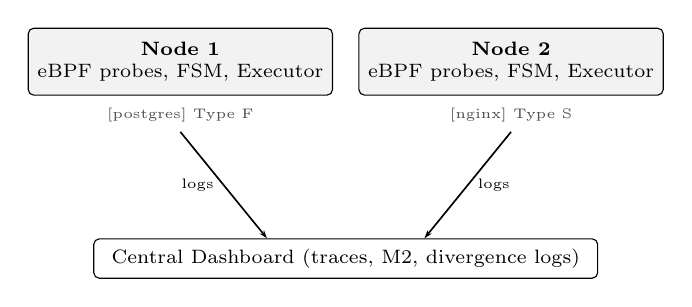
\begin{tikzpicture}[
  font=\scriptsize,
  nbox/.style={draw, rounded corners=2pt, minimum width=2.8cm,
               minimum height=0.85cm, align=center, fill=gray!10},
  wide/.style={draw, rounded corners=2pt, minimum width=6.4cm,
               minimum height=0.50cm, align=center, fill=white},
  arr/.style={-{Stealth[length=3pt, width=2pt]}, line width=0.6pt},
  wlabel/.style={font=\tiny, text=black!70},
]
\node[nbox] (n1) at (-2.1, 2.2)
  {\textbf{Node 1}\\eBPF probes, FSM, Executor};
\node[nbox] (n2) at ( 2.1, 2.2)
  {\textbf{Node 2}\\eBPF probes, FSM, Executor};
\node[wlabel, below=1pt of n1] (w1) {[postgres] Type~F};
\node[wlabel, below=1pt of n2] (w2) {[nginx] Type~S};
\node[wide] (dash) at (0, -0.3)
  {Central Dashboard \normalfont(traces, M2, divergence logs)};
\draw[arr] (w1.south) -- ([xshift=-1.0cm]dash.north)
  node[pos=0.5, left, font=\tiny] {logs};
\draw[arr] (w2.south) -- ([xshift=1.0cm]dash.north)
  node[pos=0.5, right, font=\tiny] {logs};
\end{tikzpicture}
\caption{Target Kubernetes deployment. Each node runs a DaemonSet
pod with local probes and FSM instances; only traces and
divergence metrics flow to the central dashboard.}
\label{fig:k8s}
\end{figure}

\section{Conclusion}
\label{sec:conclusion}

Separating stateless and stateful containers onto parallel eBPF-driven control paths lets each track enforce only the constraints its failure semantics require. Stateless workloads carry no persistent state that an ill-timed restart could damage, so Type~S needs only a threshold DAG. Type~F adds a five-state FSM and WASM policy layer to enforce action sequencing and block \texttt{checkpoint\_and\_restart} until the audit phase completes. Executing each reconcile cycle on both the live FSM and a throwaway instance makes the FSM's effect on dispatch decisions directly observable.

The ablation confirms that neither a stateless policy nor a memoryless baseline replicates the full system's behaviour---the two failure modes are complementary, not equivalent. FSM state persistence, WASM gating, and shadow execution together impose overhead that is negligible at the 5\,s operational timescale. New policy modules can be added to the WASM layer without touching the FSM transition relation, and the divergence metric M2 offers a continuous, interpretable signal for monitoring control-plane health post-deployment. Together, these properties make the dual-track architecture practical for production environments where stateless and stateful workloads coexist.

\begin{thebibliography}{00}

\bibitem{b14}
K. Rzadca, P. Findeisen, J. \'{S}widerski, P. Zych, P. Broniek, J. Ku\'{s}mierek, P. Nowak, B. Strack, P. Witusowski, S. Hand, and J. Wilkes, ``Autopilot: workload autoscaling at Google,'' in \textit{Proc. 15th European Conf. Computer Systems (EuroSys)}, Apr.\ 2020, doi: 10.1145/3342195.3387524.

\bibitem{b1}
B. Burns, B. Grant, D. Oppenheimer, E. Brewer, and J. Wilkes, ``Borg, Omega, and Kubernetes: Lessons learned from three container-management systems over a decade,'' \textit{ACM Queue}, vol.~14, no.~1, pp.~70--93, Mar.\ 2016, doi: 10.1145/2898442.2898444.

\bibitem{b6}
B. Gregg, \textit{BPF Performance Tools: Linux System and Application Observability}. Boston, MA: Addison-Wesley Professional, 2019.

\bibitem{b15}
N. Bronson, A. Aghayev, A. Charapko, and T. Zhu, ``Metastable failures in distributed systems,'' in \textit{Proc. Workshop on Hot Topics in Operating Systems (HotOS)}, 2021, doi: 10.1145/3458336.3465286.

\bibitem{b8}
J.~O. Kephart and D.~M. Chess, ``The vision of autonomic computing,'' \textit{Computer}, vol.~36, no.~1, pp.~41--50, Jan.\ 2003, doi: 10.1109/MC.2003.1160055.

\bibitem{b7}
IBM Corporation, ``An architectural blueprint for autonomic computing,'' IBM White Paper, 4th~ed., Jun.\ 2006.

\bibitem{b10}
C. Cao, A. Blaise, S. Verwer, and F. Rebecchi, ``Learning state machines to monitor and detect anomalies on a Kubernetes cluster,'' in \textit{Proc. 17th Int. Conf. Availability, Reliability and Security (ARES)}, 2022, Art. no.~117, pp.~117:1--117:9, doi: 10.1145/3538969.3543810.

\bibitem{b3}
A. Basiri, N. Behnam, R. de Rooij, L. Hochstein, L. Kosewski, J. Reynolds, and C. Rosenthal, ``Chaos engineering,'' \textit{IEEE Software}, vol.~33, no.~3, pp.~35--41, May/Jun.\ 2016, doi: 10.1109/MS.2016.60.

\bibitem{b9}
L. Lamport, \textit{Specifying Systems: The TLA+ Language and Tools for Hardware and Software Engineers}. Boston, MA: Addison-Wesley, 2002.

\bibitem{b11}
A. Haas, A. Rossberg, D.~L. Schuff, B.~L. Titzer, M. Holman, D. Gohman, L. Wagner, A. Zakai, and J.~F. Bastien, ``Bringing the web up to speed with WebAssembly,'' in \textit{Proc. 38th ACM SIGPLAN Conf. Programming Language Design and Implementation (PLDI)}, Jun.\ 2017, pp.~185--200, doi: 10.1145/3062341.3062363.

\bibitem{b4}
Wasmtime Contributors, ``Wasmtime: A fast and secure runtime for WebAssembly,'' [Online]. Available: \url{https://wasmtime.dev}. [Accessed: 04 Apr. 2026].

\bibitem{b2}
CRIU Project, ``CRIU: Checkpoint/Restore In Userspace,'' [Online]. Available: \url{https://criu.org}. [Accessed: 20 Jun. 2026].

\bibitem{b12}
X. Sun, W. Luo, J.~T. Gu, A. Ganesan, R. Alagappan, M. Gasch, L. Suresh, and T. Xu, ``Automatic reliability testing for cluster management controllers,'' in \textit{Proc. 16th USENIX Symp. Operating Systems Design and Implementation (OSDI)}, Jul.\ 2022.

\bibitem{b16}
Y. He, R. Guo, Y. Xing, X. Che, K. Sun, Z. Liu, K. Xu, and Q. Li, ``Cross container attacks: The bewildered eBPF on clouds,'' in \textit{Proc. 32nd USENIX Security Symp.}, Aug.\ 2023.

\bibitem{b13}
X. Sun, W. Ma, J.~T. Gu, Z. Ma, T. Chajed, J. Howell, A. Lattuada, O. Padon, L. Suresh, A. Szekeres, and T. Xu, ``Anvil: Verifying liveness of cluster management controllers,'' in \textit{Proc. 18th USENIX Symp. Operating Systems Design and Implementation (OSDI)}, Jul.\ 2024.

\end{thebibliography}

\end{document}
